\section{StartupBench}


%已润色一遍，表格需要填好。



\begin{table}[t]
\caption{Comparison of StartupBench with existing benchmarks. E2E denotes end-to-end workflow completion; Item-wise Eval. denotes criterion-level judging. \cmark, \xmark, and \pmark indicate full, no, and partial support.}
\label{tab:main_stat}
\centering
\resizebox{\textwidth}{!}{
\begin{tabular}{lccccccc}
\toprule
\textbf{Benchmark} &
\textbf{\thead{Task Source}} &
\textbf{\thead{Final \\ Output}} &
\textbf{E2E} &
\textbf{\thead{Item-wise \\ Eval.}} &
\textbf{\thead{Process \\ Logic}} &
\textbf{\thead{Open-\\ended}} &
\textbf{\thead{Evaluation \\ Method}} \\
\midrule


GAIA \citep{mialon2024gaia}
& Manual
& Text
& \pmark
& \xmark
& \xmark
& \xmark
& Rule \\

OSWorld \citep{xieosworld}
& Real+Manual
& Env State
& \pmark
& \xmark
& \xmark
& \xmark
& Execution \\

DAComp \citep{lei2025dacomp}
& Real+Manual
& Workspace
& \cmark
& \xmark
& \xmark
& \cmark
& Hybrid \\



GDPval \citep{patwardhan2025gdpval}
& Manual
& Work products
& \cmark
& \xmark
& \xmark
& \pmark
& Manual \\

Workspace-Bench \citep{tang2026workspace}
& Sim.+Manual
& Workspace
& \cmark
& \xmark
& \xmark
& \cmark
& Agent-as-Judge \\

OneMillionBench \citep{yang2026onemillion}
& Expert-authored
& Text
& \pmark
& \xmark
& \pmark
& \cmark
& LLM-judge \\

Agents' Last Exam \citep{sun2026agents}
& Occupation-guided
& Workspace
& \cmark
& \xmark
& \pmark
& \pmark
&  Hybrid \\

OfficeQA Pro \citep{opsahl2026officeqa}
& Corpus-grounded
& Text
& \xmark
& \xmark
& \xmark
& \xmark
& Answer match \\

\midrule

\textbf{StartupBench (Ours)}
& \textbf{\thead{Market-vetted\\+ Expert-built}}
& \textbf{Workspace}
& \cmark
& \cmark
& \cmark
& \cmark
& \textbf{Agent-as-Judge} \\

\bottomrule
\end{tabular}
}
\end{table}



\begin{figure*}[t]
    \centering
    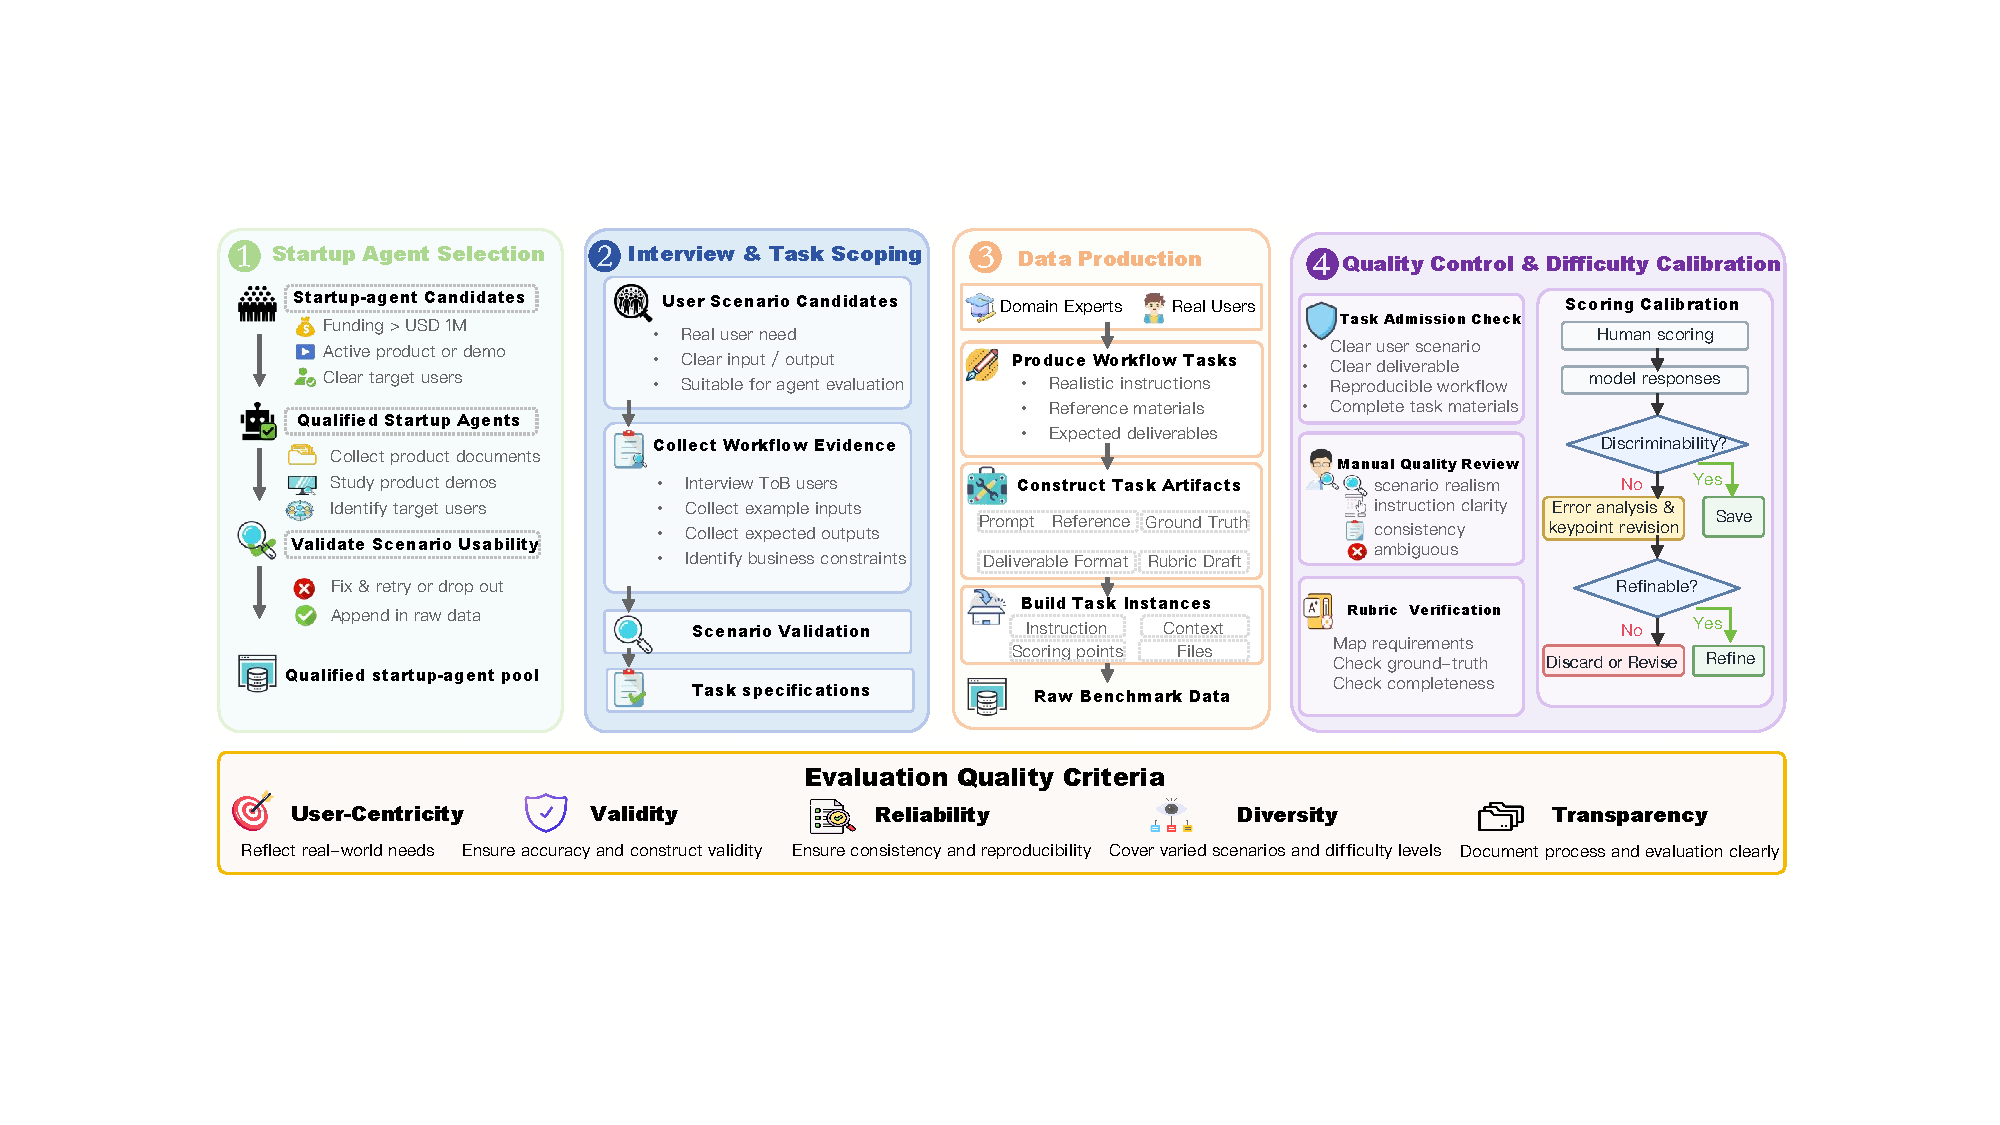
\includegraphics[width=0.99\textwidth]{figures/StartupBench-fig2.pdf}
    \caption{
    StartupBench data construction pipeline. We select market-validated startup agents, collect real user workflows, construct task artifacts and instances, and calibrate quality and difficulty through multi-stage review.
    }
    \label{fig:data_workflow}
% \vspace{-6pt}
\end{figure*}



StartupBench is designed to evaluate whether models and agents can complete realistic workflows that users already delegate to AI products. This objective requires data that reflects authentic user demand while supporting controlled evaluation. We therefore require each task to be realistic, answerable, evaluable, and discriminative: it should originate from actual AI product usage, provide sufficient information for a valid solution, specify clear output requirements and assessment criteria, and remain challenging enough to distinguish current models and agents.

Neither manual task design nor direct extraction from product demonstrations is sufficient to obtain such data. The former is controllable but may be detached from real demand, while the latter is realistic but often lacks context, success criteria, or reproducible specifications. We therefore adopt a survey- and interview-driven multi-stage pipeline shown in Figure~\ref{fig:data_workflow}.  We first survey market-validated AI-native startups, interview deep users to identify usage contexts, task goals, and expected deliverables, recruit domain experts to convert validated scenarios into benchmark instances, and finally apply quality control for realism, answerability, evaluability, and discriminative difficulty.
\subsection{Dataset Construction}

\subsubsection{Startup Survey for Market-Validated Agent Scenarios}

We first survey AI-native startups that build agent products across diverse domains. To identify workflows with market validation, we retain startups with more than USD 1M in funding and require evidence of real adoption, either through paid usage or substantial user traction. Funding provides a coarse signal of market expectation, while payment or user-scale evidence indicates that the product is used beyond exploratory demonstrations. The output of this stage is a pool of candidate products and workflows for user interviews. During this stage we collect 20+ start-up agents as the basis for subsequent stage.

\subsubsection{User Interviews for Scenario and Requirement Discovery}

For each candidate Startup-product, we interview deep users of the corresponding agent from different domains to recover practical usage beyond public product descriptions. The interviews elicit the usage context, user goal, input information, expected deliverable, success criteria, and common constraints. We summarize these findings into scenario specifications and representative demo cases, which serve as anchors for later annotation stage.
During this stage we interview over 30 deep users and collected at least one demo case for each candidate Agent.


\subsubsection{Expert Construction of Domain Tasks}



Given the interview-derived workflow specifications and representative user scenarios as a reference or seed task, we recruit over 50 domain experts to reconstruct benchmark tasks that preserve the original workflow objectives, practical constraints, and expected deliverables while adapting them into reproducible evaluation instances. Rather than designing synthetic problems, experts standardize authentic user requests into benchmark tasks that faithfully represent real professional workflows.

Every task is required to satisfy three principles: it must originate from a realistic work request that users would naturally delegate to AI agents, involve an end-to-end workflow rather than an isolated subtask, and produce concrete professional deliverables with clearly defined success criteria and fine-grained evaluation rubrics for objective evaluation.

To standardize these tasks for evaluation, each task is represented as a triple
\[
\mathcal{T}=(q,\mathcal{E},\mathcal{R}),
\]
where $q$ is a natural-language user request describing the task, $\mathcal{E}$ denotes the workspace containing all input files and resources required to complete the task, and $\mathcal{R}=\{(p_i,w_i)\}_{i=1}^{n}$ is a set of weighted evaluation rubrics that assess complementary aspects of deliverable quality. Detailed task specifications and annotation guidelines are provided in Appendix~\ref{app:task_construction}. During this stage, we collect over 150 candidate tasks for further quality control.







\subsubsection{Quality Control}
To ensure benchmark quality and consistency, every task undergoes the following multi-stage quality control process:

\textbf{Expert Cross Validation.}
Every task is independently reviewed by at least one additional domain expert.
Reviewers verify four aspects of task quality:
(1) the authenticity and correctness of the task description and workspace,
(2) the fidelity of the reconstructed workflow,
(3) the validity of the evaluation rubrics, and
(4) the consistency between the reference deliverable and the finalized evaluation protocol.
Detailed review criteria are provided in Appendix~\ref{app:cross_valid}.





\textbf{Difficulty Control.}We calibrate task difficulty through pilot executions using several frontier models under the same evaluation harness adopted in the benchmark\footnote{We randomly select models from GPT-5.5, Seed-2.1-Pro and GLM-5.1 as the model for pilot executions, intending to construct a challenging and discriminative benchmark rather than to estimate performance over the natural task distribution.}. Tasks that are consistently completed with high quality are excluded due to limited discriminative value. Pilot results also serve as an additional quality assurance stage: when failures are attributed to ambiguous instructions, incomplete workspace information, or inadequately specified evaluation criteria rather than intrinsic task difficulty, the corresponding task is revised and re-validated before inclusion.


\subsection{Statistics for StartupBench}

\textbf{StartupBench} contains 97 real-world workflow tasks across 6 top-level domains: Medical \& HealthCare, Finance, Legal, Business \& Management, STEM \& Computer Science, and Education \& Humanities. These tasks are designed to reflect deliverable-oriented workflows in realistic office settings, requiring agents to understand task contexts, follow complex constraints, process heterogeneous files, and produce usable work products. For evaluation, each task is evaluated using an average of \textbf{25.3} fine-grained rubrics, spanning \textbf{6 dimensions and 3 importance levels} , enabling detailed assessment of complex, long-horizon workflows and diverse work deliverables. The  summary of the domain coverage and main output formats of StartupBench is shown in Table~\ref{tab:benchmark_statistics}.


\begin{table}[t]
\centering
\small
\setlength{\tabcolsep}{12pt}
\renewcommand{\arraystretch}{1.12}
\begin{threeparttable}
\caption{Statistics of StartupBench. The benchmark contains 97 real-world workflow tasks across six top-level domains and requires diverse deliverable formats.}
\label{tab:benchmark_statistics}

\begin{tabular}{l S[table-format=3.0] S[table-format=3.1]}
\toprule
\textbf{Category} & {\textbf{Count}} & {\textbf{Percentage (\%)}} \\
\midrule

\rowcolor{gray!8}
\multicolumn{3}{l}{\textit{Overall statistics}} \\
Total tasks & 97 & 100.0 \\
Top-level domains & 6 & \multicolumn{1}{c}{--} \\

\midrule
\rowcolor{gray!8}
\multicolumn{3}{l}{\textit{Domain distribution}} \\
Medical \& HealthCare & 21 & 21.6 \\
Finance & 18 & 18.6 \\
Legal & 16 & 16.5 \\
Business \& Management & 19 & 19.6 \\
STEM \& Computer Science & 16 & 16.5 \\
Education \& Humanities & 7 & 7.2 \\

\bottomrule
\end{tabular}

\begin{tablenotes}[flushleft]
\footnotesize
\item \textit{Output formats:} DOCX, XLSX, PPTX, PDF, Markdown, images, and text-based deliverables.
\end{tablenotes}
\end{threeparttable}
\end{table}





\subsection{Automatic Evaluation of StartupBench Tasks}

As stated above, every task in StartupBench is defined as a triple $\mathcal{T}=(q,\mathcal{E},\mathcal{R})$. Given $(q,\mathcal{E})$, the evaluated model produces a set of deliverables $\mathcal{D}$. Before evaluation, we construct a lightweight evidence view $\mathcal{V}(\mathcal{D})$, consisting of extracted textual content and rendered page images, to facilitate navigation over heterogeneous artifacts while allowing the judge to access the original files whenever necessary.

Rather than relying on a single holistic judgment, StartupBench evaluates each rubric item independently through a dedicated AgentJudge session. Most tasks contain 20+ fine-grained rubric items covering diverse aspects of the expected deliverables, including functionality, completeness, formatting, and domain-specific requirements. Evaluating these criteria separately allows each rubric to receive dedicated reasoning and tool usage without interference from unrelated evaluation dimensions, while ensuring that every requirement is assessed explicitly. The final task score is then obtained by aggregating the outcomes of all rubric-level evaluations.

Following \textbf{Agent-as-a-Judge}, each rubric evaluation is carried out by a lightweight agent rather than a single forward pass. Let $J$ denote the judging prompt and evaluation protocol used by the AgentJudge, given the task specification, deliverables, evidence view, and the target rubric item $p_i$, the judge produces both a binary decision $y_i\in\{0,1\}$ indicating whether the rubric is satisfied and a textual justification $e_i$:

\begin{equation}
(y_i,e_i) = \mathrm{AgentJudge}\big(J, q,
\mathcal{D}, \mathcal{V}(\mathcal{D}), p_i\big),
\label{eq}
\end{equation}

The final task score is computed by aggregating the weighted decisions across all rubric items:

\begin{equation}
\mathrm{score}(\mathcal{D},\mathcal{T})
= \frac{\sum_{i=1}^{n} w_i y_i}{\sum_{i=1}^{n} w_i}
\in [0,1].
\label{eq2}
\end{equation}
%\subsection{Hello World}